\begin{question}{20}{
    Tijdens een trainingsdag wordt een alarmsituatie gehouden op de Trip van Zoudtlandtkazerne.
    Van \'e\'en peloton worden de reactietijden (in seconden) gemeten tussen het afgaan van het alarm en het moment dat de militair volledig gevechtsgereed is.

    De gemeten reactietijden van de militairen in het peloton zijn als volgt:
    \[
        18,\; 21,\; 19,\; 25,\; 23,\; 22,\; 20,\; 24,\; 26,\; 19,\; 21,\; 23,\; 27,\; 30,\; 18,\; 22,\; 24,\; 35,\; 28,\; 20.
    \]
}
        \subquestion{10}{
            Teken een boxplot van de reactietijden.
            Schrijf hierbij de stappen op die je hebt uitgevoerd om de vijf getallen voor de boxplot te kunnen bepalen.
        }
        \solution{
            Om de vijf getallen voor de boxplot te bepalen, volgen we de volgende stappen:
            \begin{itemize}
                \item Sorteer de gegevens van laag naar hoog:
                \[
                    18,\; 18,\; 19,\; 19,\; 20,\; 20,\; 21,\; 21,\; 22,\; 22,\; 23,\; 23,\; 24,\; 24,\; 25,\; 26,\; 27,\; 28,\; 30,\; 35. \rubric{1}
                \] 
                \item De minimumwaarde is $18$ en de maximumwaarde is $35$.\rubric{1}
                \item Aangezien het aantal waarden $n = 20$, dus $n$ is even, is de mediaan (tweede kwartiel) het gemiddelde van de twee middelste waarden: $\frac{22 + 23}{2} = 22.5$.\rubric{1}
                \item Het eerste kwartiel $Q_1$ is de mediaan van de laagste \SI{50}{\percent} waarden ($18, 18, 19, 19, 20, 20, 21, 21, 22, 22$).
                Aangezien er $10$ waarden zijn, is het eerste kwartiel het gemiddelde van de vijfde en zesde waarde: $Q_1=\frac{20 + 20}{2} = 20$.\rubric{2}
                \item Het derde kwartiel $Q_3$ is de mediaan van de laagste \SI{50}{\percent} waarden ($23, 23, 24, 24, 25, 26, 27, 28, 30, 35$).
                Aangezien er $10$ waarden zijn, is het derde kwartiel het gemiddelde van de vijfde en zesde waarde: $Q_3=\frac{25 + 26}{2} = 25.5$.\rubric{1}
            \end{itemize}
            De vijf getallen voor de boxplot zijn dus:
            \[
                \text{Minimum} = 18, \quad Q_1 = 20, \quad \text{Mediaan} = 22.5, \quad Q_3 = 25.5, \quad \text{Maximum} = 35. 
            \]
            
            We tekenen de boxplot met snorharen van $Q_1 - 1.5 \times \IQR$ tot $Q_3 + 1.5 \times \IQR$, waarbij $\IQR = Q_3 - Q_1 = 25.5 - 20 = 5.5$. \rubric{1}
            De \enquote{whiskers} lopen van de kleinste niet-outlier boven $20 - 1.5 \times 5.5 = 11.75$ (oftewel $18$) tot de hoogste niet-outlier onder $25.5 + 1.5 \times 5.5 = 33.75$ (oftewel $30$).
            Er is één outlier, namelijk $35$. \rubric{1}
            \begin{center}
                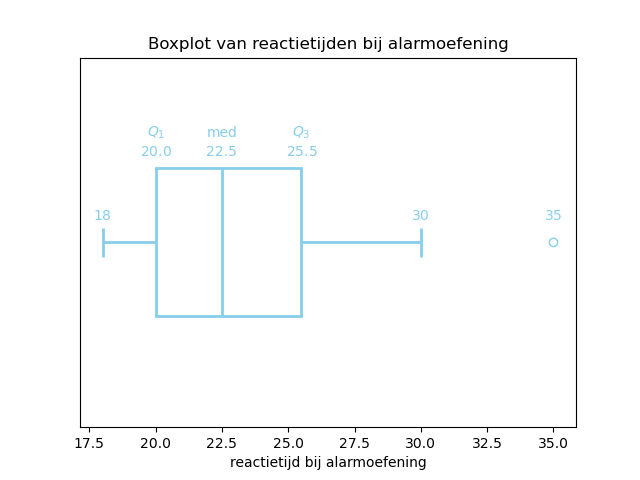
\includegraphics[width=\textwidth]{./20260605_exam_boxplot.png} \rubric{2}
            \end{center}

        }

        \subquestion{3}{
            Leg met behulp van de boxplot uit wat je kunt zeggen over de ligging van het gemiddelde ten opzichte van de mediaan?
        }
        \solution{
            Aan de boxplot is te zien dat de data een positieve scheefheid vertoont.\rubric{1}
            Dit is te zien aan de langere snorhaar aan de rechterkant van de boxplot en de aanwezigheid van een outlier aan de rechterkant.
            In een positief scheve verdeling ligt het gemiddelde hoger dan de mediaan, omdat het gemiddelde wordt beïnvloed door de hogere waarden (zoals de outlier $35$).\rubric{1}
            Daarom kunnen we concluderen dat het gemiddelde van de reactietijden hoger ligt dan de mediaan van $22.5$ seconden. \rubric{1}
        }
        \subquestion{2}{
            Noem \'e\'en reden waarom deze steekproef mogelijk niet representatief is voor de reactietijden van alle militairen in de Trip van Zoudtlandtkazerne.
        }
        \solution{
            Een mogelijke reden waarom deze steekproef niet representatief is, is dat de reactietijden alleen zijn gemeten van \'e\'en specifiek peloton.\rubric{1}
            De reactietijden kunnen variëren tussen verschillende pelotons vanwege verschillen in training, ervaring of andere factoren.
            Hierdoor zou de resultaten van deze steekproef mogelijk niet generaliseerbaar kunnen zijn naar alle militairen in de Trip van Zoudtlandtkazerne. \rubric{1}
        }

        \subquestion{5}{
            Tijdens de analyse ontdekt men dat er een fout is gemaakt bij het invoeren van de reactietijd van een van de militairen, en dat deze reactietijd eigenlijk $40$ seconden had moeten zijn in plaats van $30$ seconden. Geef aan wat er zou veranderen aan de boxplot als deze fout wordt gecorrigeerd.
        }
        \solution{
            Als de fout wordt gecorrigeerd en de reactietijd van $30$ seconden wordt vervangen door $40$ seconden, zal dit de maximumwaarde in de dataset veranderen van $35$ naar $40$.\rubric{1}
            De minimumwaarde, het eerste kwartiel, de mediaan en het derde kwartiel zullen echter niet veranderen, omdat deze waarden niet worden beïnvloed door de hoogste waarde in de dataset.\rubric{2}
            De whisker aan de rechterkant van de boxplot zal nu lopen tot de hoogste niet-outlier onder $25.5 + 1.5 \times 5.5 = 33.75$, oftewel $28$, en er zullen nu twee outliers zijn: $35$ en $40$. \rubric{2}
            \begin{center}
                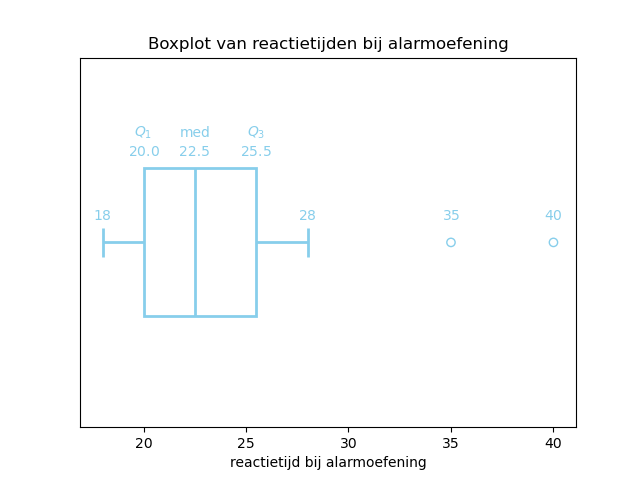
\includegraphics[width=\textwidth]{./20260605_exam_boxplot2.png}
            \end{center}
        }
\end{question}